%%%%%%%%%%%%%%%%%%%%%%%%%%%%%%%%%%%%%%%%%
% Structured General Purpose Assignment
% LaTeX Template
%
% This template has been downloaded from:
% http://www.latextemplates.com
%
% Original author:
% Ted Pavlic (http://www.tedpavlic.com)
%
% Note:
% The \lipsum[#] commands throughout this template generate dummy text
% to fill the template out. These commands should all be removed when 
% writing assignment content.
%
%%%%%%%%%%%%%%%%%%%%%%%%%%%%%%%%%%%%%%%%%

%----------------------------------------------------------------------------------------
%   PACKAGES AND OTHER DOCUMENT CONFIGURATIONS
%----------------------------------------------------------------------------------------

\documentclass{article}

\usepackage{fancyhdr} % Required for custom headers
\usepackage{lastpage} % Required to determine the last page for the footer
\usepackage{extramarks} % Required for headers and footers
\usepackage{graphicx} % Required to insert images
\usepackage{lipsum} % Used for inserting dummy 'Lorem ipsum' text into the template

\usepackage[T1]{fontenc} % Codificación de las fuentes utilizadas
\usepackage[spanish]{babel} % Español como idioma principal del texto (permite hyphenation de palabras al final de una línea)
\selectlanguage{spanish}
\usepackage{hyperref}
\usepackage{listings}

\usepackage[T1]{fontenc} % Codificación de las fuentes utilizadas
\usepackage[spanish]{babel} % Español como idioma principal del texto (permite hyphenation de palabras al final de una línea)


\usepackage{graphicx}
\usepackage{url}

\graphicspath{{Figures/}{Diagrams}{Chapters/}}  % Location of the graphics files (set up for graphics to be in PDF format)

\selectlanguage{spanish}

\setcounter{tocdepth}{1}

% Include any extra LaTeX packages required
\usepackage[square, numbers, comma, sort&compress]{natbib}  % Use the "Natbib" style for the references in the Bibliography
\usepackage{verbatim}  % Needed for the "comment" environment to make LaTeX comments
\usepackage{vector}  % Allows "\bvec{}" and "\buvec{}" for "blackboard" style bold vectors in maths
\hypersetup{urlcolor=blue, colorlinks=true}  % Colours hyperlinks in blue, but this can be distracting if there are many links.
\usepackage{hyperref}
% \usepackage[pdfauthor={Diego Martín Arroyo},
%             pdftitle={Diseño e implementación de un sistema de computación distribuida con
% Raspberry Pi, y estudio comparativo del mismo frente a otras soluciones},
%             pdfsubject={Memora del Trabajo de Fin de Grado},
%             pdfproducer={XeLaTeX with hyperref},
%             pdfcreator={XeLaTeX},
%             pdfkeywords={Computación Paralela, Sistema Distribuido, Raspberry}
%             ]{hyperref}
%% ----------------------------------------------------------------

%% --------------------------------------------------------------------------------------------------------------------------------
%http://tex.stackexchange.com/a/85218/76599
\usepackage{fancyvrb}
\usepackage[dvipsnames]{xcolor}

% redefine \VerbatimInput
\RecustomVerbatimCommand{\VerbatimInput}{VerbatimInput}% Inclusión de archivos de texto plano
{fontsize=\footnotesize,
 %
 frame=lines,  % top and bottom rule only
 framesep=2em, % separation between frame and text
 rulecolor=\color{Gray},
 %
 label=\fbox{\color{Black}data.txt},
 labelposition=topline,
 %
 commandchars=\|\(\), % escape character and argument delimiters for
                      % commands within the verbatim
 commentchar=*        % comment character
}

\usepackage{listings} % Requerido para la inserción de código
%Listings command

\usepackage{float}
\newcommand*\lstinputpath[1]{\lstset{inputpath=#1}}
\lstinputpath{Code/}

\newcounter{undefinedreferences}
\setcounter{undefinedreferences}{0}

\newcommand{\citationneeded}[1][None]{\stepcounter{undefinedreferences}\textsuperscript{\color{blue} [Citation needed: #1]}}

\newcommand{\checkreferences}{
\ifnum\value{undefinedreferences} > 0
\begin{center}
\immediate\write18{wget -O Figures/protester.png -nc http://imgs.xkcd.com/comics/wikipedian_protester.png}
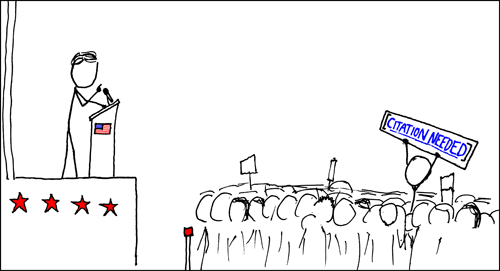
\includegraphics[width=\textwidth]{protester.png}\\
There are \arabic{undefinedreferences} undefined references
\end{center}
\else
No undefined references. Good!
\fi
}


%https://github.com/pads-fhs/LaTeX-Template-Thesis/blob/master/lststyles.tex
\lstdefinelanguage{JavaScript}{
  keywords={typeof, new, true, false, catch,%
    function, return, null, catch, switch, var,%
    if, in, while, do, else, case, break},
  ndkeywords={class, export, boolean, throw, implements, import, this},
  sensitive=false,
  comment=[l]{//},
  morecomment=[s]{/*}{*/},
  morestring=[b]',
  morestring=[b]"
}
\newcommand{\lstsetjavascript}{
  \lstset{
		language=JavaScript,
		breaklines=true,
		commentstyle=\textit,
		basicstyle=\ttfamily,
		keywordstyle=\bfseries,
		stringstyle=\ttfamily,
		showstringspaces=false,
		frame=single,
		tabsize=2
  }
}

\lstdefinelanguage{log}{
  keywords={typeof, new, true, false, catch,%
    function, return, null, catch, switch, var,%
    if, in, while, do, else, case, break},
  ndkeywords={class, export, boolean, throw, implements, import, this},
  sensitive=false,
  comment=[l]{//},
  morecomment=[s]{/*}{*/},
  morestring=[b]',
  morestring=[b]"
}
\newcommand{\lstsetlog}{
  \lstset{
		language=log,
		breaklines=true,
		commentstyle=\textit,
		basicstyle=\ttfamily,
		keywordstyle=\bfseries,
		stringstyle=\ttfamily,
		showstringspaces=false,
		frame=single,
		tabsize=2
  }
}

\lstloadlanguages{Java,XML, JavaScript, log}

\newcommand{\javascriptcode}[4]{
	\lstinputlisting[caption=#2,label=#1, firstline=#3, lastline=#4]{#1.json}
}

\newcommand{\logcode}[4]{
	\lstinputlisting[caption=#2,label=#1, firstline=#3, lastline=#4]{#1.log}
}

\usepackage[bottom]{footmisc} %The footnotes go at the bottom of t\usepackage{dtklogos}he page, instead next to the last line.
%Ajustes para Java
% \lstset{
% 	language=java,
%  	frame=single, % Un marco simple alrededor del código
%     basicstyle=\small\ttfamily, % Utilizar fuente true type pequeña
%     keywordstyle=[1]\color{Blue}\bf, % Funciones en negrita y azul
%     keywordstyle=[2]\color{Purple}, % Argumentos en morado
%     keywordstyle=[3]\color{Blue}\underbar, % Funciones personalizadas subrayadas en azul
%     identifierstyle=, % Nada especial acerca de identificadores
%     commentstyle=\usefont{T1}{pcr}{m}{sl}\color{Green}\small, % Los comentarios se renderizan en fuente pequeña verde
%     stringstyle=\color{Purple}, % Cadenas en morado
%     showstringspaces=false, % No se muestran los espacios entre cadenas
%     tabsize=5, % 5 espacios por tabulado
%     %
%     % Put standard Perl functions not included in the default language here
%     %morekeywords={rand},
%     %
%     % Put Perl function parameters here
%     %morekeywords=[2]{on, off, interp},
%     %
%     % Put user defined functions here
%     %morekeywords=[3]{test},\usepackage{dtklogos}
%    	%
%     morecomment=[l][\color{Blue}]{...}, % Line continuation (...) like blue comment
%     numbers=left, % Número de línea a la izquierda
%     firstnumber=1, % Número de línea comienza en 1
%     numberstyle=\tiny\color{Blue}, % Los números de línea son azules y pequeños
%     stepnumber=5, % Los números de línea van de 5 en 5
%     breaklines=true % Salto de línea si el texto no entra. See http://stackoverflow.com/a/1875803
% }

%\usepackage{xltxtra} % XeLaTeX logo. Yep, just that
%http://tex.stackexchange.com/a/73179/76599
\usepackage{metalogo}
%\usepackage{dtklogos} %BibTeX logo
\def\BibTeX{{\rm B\kern-.05em{\sc i\kern-.025em b}\kern-.08em
    T\kern-.1667em\lower.7ex\hbox{E}\kern-.125emX}}

\newenvironment{alignedDescription}[2][0pt]
  {\begin{list}{}%
    {\renewcommand\makelabel[1]{\textsf{\textbf{##1}}\hfil}%
     \settowidth\labelwidth{\makelabel{#2}}%
     \setlength\leftmargin{\labelwidth+\labelsep + #1}}}%
  {\end{list}}

\newenvironment{elements}
{\begin{quote}\itshape\centering\small}
{\end{quote}}

\newenvironment{cabstract}
{\begin{quote}\itshape\centering\small}
{\end{quote}}

%\usepackage[xindy]{glossaries}
%\newcommand{\chapterabstract}{1}{
%	\begin{center}
%	\small\textit
%	#1
%	\end{center}
%}

\usepackage{xcolor,colortbl}
   
%----------------------------------------------------------------------------------------
%   NAME AND CLASS SECTION
%----------------------------------------------------------------------------------------

\newcommand{\hmwkTitle}{Configuración de la autenticación del sistema} % Assignment title
\newcommand{\hmwkDueDate}{Miércoles,\ 29\ de\ April\ de\ 2015} % Due date
\newcommand{\hmwkAuthorName}{Diego Martín Arroyo} % Your name

%----------------------------------------------------------------------------------------
%   TITLE PAGE
%----------------------------------------------------------------------------------------

\title{\hmwkTitle}
\author{\textbf{\hmwkAuthorName}}
\date{21 de abril de 2015}

%----------------------------------------------------------------------------------------

\begin{document}

\maketitle

%----------------------------------------------------------------------------------------
%   TABLE OF CONTENTS
%----------------------------------------------------------------------------------------

\setcounter{tocdepth}{1}

\newpage
\tableofcontents
\newpage

\section{Introducción}

La infraestructura en la que se integra el sistema a construir cuenta con un sistema de usuarios centralizado en un servidor \textit{LDAP} (\textit{Lightweight Directory Access Protocol}), que posibilita el almacenamiento centralizado de la información de todos los usuarios de la infraestrucutra, y que, combinado con otros componentes, permite la utilización de una única cuenta en cualquiera de los equipos de la misma. Este sistema proporciona una serie de ventajas: delega la gestión de los usuarios al sistema central y evita la creación de nuevas cuentas para cada usuario, evitando el procesado de una cantidad de usuarios significativa.

Es por ello que el sistema contará con un cliente \textbf{LDAP} en cada uno de los nodos para poder acceder a la cuenta de cada usuario.

\section{LDAP}

El protocolo abierto \textbf{LDAP} se basa en una arquitectura cliente-servidor. En dicha arquitectura, el servidor gestiona un directorio de usuarios con una serie de datos de relevancia, tales como el par de claves usuario-contraseña, nombre completo, directorio de inicio, \textit{shell} por defecto, etcétera. La versión actual del protocolo (versión 3) se define en \cite{rfc4511} 

\subsection{Servidor a utilizar}

El servidor \textbf{LDAP} presente en la infraestructura utiliza una configuración estándar accesible desde la URI  \texttt{ldap://ldap1.cie.aulas.usal.es}. No utiliza autenticación por TLS \textit{Transport Layer Security} y opera en el puerto por defecto del protocolo, el 389.

\section{Configuración}

El proceso de configuración es sencillo, y se limita a la instalación de varios paquetes y la modificación de una serie de ficheros de configuración.\\

\texttt{pacman -S openldap nss-pam-ldapd}

Para confirmar que la instalación se ha realizado de forma correcta es posible realizar consultas al servidor desde la línea de comandos:\\

\texttt{ldapsearch -x -D uid=<id>,ou=people,dc=DIA -W -H ldap://ldap1.cie.aulas.usal.es:389 -b dc=dia -s sub uid=<id>}

Si al introducir la contraseña el comando retorna la información sobre el usuario, la autenticación se ha realizado de forma exitosa. En caso contrario se retornará un código de error.

La información que provee el directorio es la siguiente:\\

%\conffile{output}{Información sobre el servidor. Obsérvese el campo base, de relevancia para la configuración del cliente}{1}{10}

En primer lugar es necesario realizar la configuración del propio cliente LDAP para poder realizar consultas al mismo, que después serán aprovechadas por otros componentes. 

\conffile{ldap}{Archivo \texttt{/etc/openldap/ldap.conf}}{1}{10}

La configuración puede probarse con el siguiente comando:\\

\texttt{ldapsearch -x `(objectclass=*)'}

\subsection{Configuración del \textit{Name Service Switch}}

Un \textbf{NSS} define un conjunto de fuentes (archivos de configuración como \texttt{/etc/passwd}, servidores externos (\textit{LDAP})) para bases de datos de configuración. Para incluir el \textbf{LDAP} como fuente de datos únicamente es necesario modificar los ficheros de configuración del mismo:

\conffile{nsswitch}{Archivo \texttt{/etc/nsswitch.conf}}{1}{19}

En el archivo \texttt{nsswitch} se incluse información como fuentes de información los archivos del sistema (\texttt{passwd}, \texttt{gpasswd}\dots) y el protocolo \textbf{LDAP}

\conffile{nslcd}{Archivo \texttt{/etc/nslcd.conf}}{1}{1}

El archivo contiene la información de acceso al servidor \textbf{LDAP}.

Una vez modificados los archivos según lo indicado, es posible comenzar a utilizar el servidor \textbf{LDAP} como método de autenticación. Para ello es necesario únicamente iniciar el servicio \texttt{nslcd} utilizando \textbf{systemd}:\\

\texttt{systemctl start nslcd}

Para comprobar el correcto funcionamiento del sistema, es posible utilizar el comando \texttt{getent passwd}, que en caso que la configuración se haya aplicado correctamente, mostrará todos los usuarios presentes en el servidor \textbf{LDAP}.

\subsection{Configuración del módulo PAM}

El \textit{Pluggable Authentication Module} (\textbf{PAM}) es un módulo que permite realizar operaciones de autenticación y gestión de sesiones y contraseñas\cite{osfrfc86} utilizando un diseño modular y ``conectable'' (\textit{pluggable}), que permite su modificación y reemplazo de forma sencilla. En \textbf{Arch Linux} el paquete que lo incluye es \texttt{nss-pam-ldapd} \cite{nss-pam-ldap}.

En general, la configuración de \textbf{PAM} consiste en añadir a los archivos de configuración presentes una serie de directivas que realicen la consulta al fichero \textbf{LDAP}. Dichos ficheros se encuentran en la ruta \texttt{/etc/pam.d}

\pamfile{pam.d/su}{Fichero \texttt{pam.d/system-auth}}{1}{20}

\pamfile{pam.d/su-l}{Ficheros \texttt{pam.d/su} y \texttt{pam.d/su-l} (su contenido es idéntico en este paso)}{1}{20}

\pamfile{pam.d/passwd}{Fichero \texttt{pam.d/passwd}}{1}{10}

\subsection{Creación del directorio de inicio}

Debido a que el directorio de inicio no entra dentro del conjunto de directorios compartidos del sistema, es necesario crearlo en caso de que el usuario acceda por primera vez al sistema. 

\pamfile{pam.d/system-login}{Fichero \texttt{pam.d/system-login}}{1}{20}
\pamfile{pam.d/su-l}{Fichero \texttt{pam.d/su-l} (obsérvese la línea de diferencia con \texttt{pam.d/su})}{1}{20}

Sin embargo esto no es suficiente para proporcionar una experiencia de uso óptima, pues la configuración descrita anteriormente no crea el directorio en el resto de nodos del sistema, obligando al usuario a iniciar sesión en cada uno de ellos para contar con un directorio de trabajo propio. Para solucionar este problema es posible utilizar un servicio de \texttt{MarcoPolo}.

También es posible dar acceso al superusuario o permitir el acceso sin conexión al servidor, de nuevo mediante parámetros de configuración.

Una vez que toda la configuración ha sido probada es posible ejecutar el comando \texttt{systemctl enable nslcd} para arrancar el sistema de autenticación cada vez que el equipo arranque.

\nocite{ldapauthenticationarch}
\nocite{openldaparch}
\nocite{openldap}

%http://www.server-world.info/en/note?os=Debian_7.0&p=ldap&f=2
%https://wiki.debian.org/LDAP/PAM
%TODO: https://wiki.archlinux.org/index.php/LDAP_Hosts

\label{Bibliography}
\lhead{\emph{Bibliography}}  % Change the left side page header to "Bibliography"
\bibliographystyle{ieeetr}  % Use the "unsrtnat" BibTeX style for formatting the Bibliography
\bibliography{ldap}  % The references (distcc) information are stored in the file named "distcc.bib"

\end{document}
